\section{PS2a: Sokaban Visual component}\label{sec:ps3a}
\graphicspath{{ps3a}}
\subsection{Discussion:}\label{sec:ps3a:disc}
The task for this project was in recreating the age-old game of Sokaban. For the first part of the assignment(a), I had to create the visual aspect. Beginning with an opague object design, I created an object for the game and had the rest of the functions within it. I did this by inheriting the public Drawable class from the SFML library, and by overloading the draw function in a virtual format. This allowed myself the ability to draw the entire class to the screen and utilize members and data structures in the process.
    
\subsection{Key algorithms, Data structures and OO Designs used in this Assignment:}\label{sec:ps3a:kdo}
The Sokaban game is inherently grid like, moving boxes around the screen to loading locations. I designed the game using an array of characters that instantiated at the start of each level, the grid included the movable locations as well as the wall locations. For the other important data points like player location, box location, and dropoff location I created different data structures to hold them including a pair of integers and two vectors consisting of pairs of integers. The first time I implemented this, I had all of the information embedded into the background grid, however I soon realized that tht it would have been difficult to model multiple figures at the same location. These pieces of data were not only dynamic, but they were a layer above the background. By removing them from the grid and giving them their own data structure I was able to always draw the background, and be able to search for their locations very easily. 

\subsection{What I learned :}\label{sec:ps2a:learn}

In this project I learned a lot about foreground and background visual effects and the utilization of different data structures to achieve the effect. I learned how to operate objected oriented design into existing libraries with the overloading of the draw function. I learned about the relationship between textures and sprites. 

\subsection{Acknowledgments :}\label{sec:ps3a:ack}
\textbf{Links :}
\begin{itemize}
    \item \url{https://www.sfml-dev.org/tutorials/2.5/graphics-sprite.php}
    \item \url{https://icarus.cs.weber.edu/~dab/cs1410/textbook/11.Operators/io_overload.html}
    \item \url{https://www.cplusplus.com/reference/vector/vector/}
    \item \url{https://www.sfml-dev.org/documentation/2.5.1/classsf_1_1Drawable.php}
    \item \url{https://stackoverflow.com/questions/34458791/making-custom-types-drawable-with-sfml}
\end{itemize}


\subsection{Codebase}\label{sec:ps2a:code}

\textbf{\colorbox{pink}{Makefile}} \newline \textbf{This Makefile has no Linting as the program does not have any lints.}
\lstinputlisting[language=Make]{ps2a/Makefile}

\textbf{\colorbox{pink}{main.cpp}} \newline 
\lstinputlisting{ps2a/main.cpp}

\textbf{\colorbox{pink}{Sokoban.h}} \newline \
\lstinputlisting{ps2a/Sokoban.h}

\newpage
\textbf{\colorbox{pink}{Sokoban.cpp}} \newline \lstinputlisting{ps2a/Sokoban.cpp}
\lstinputlisting{ps2a/Sokoban.cpp}

\newpage
\subsection{Output:}\label{sec:ps2a:output}
\begin{figure}[h]
    \centering
    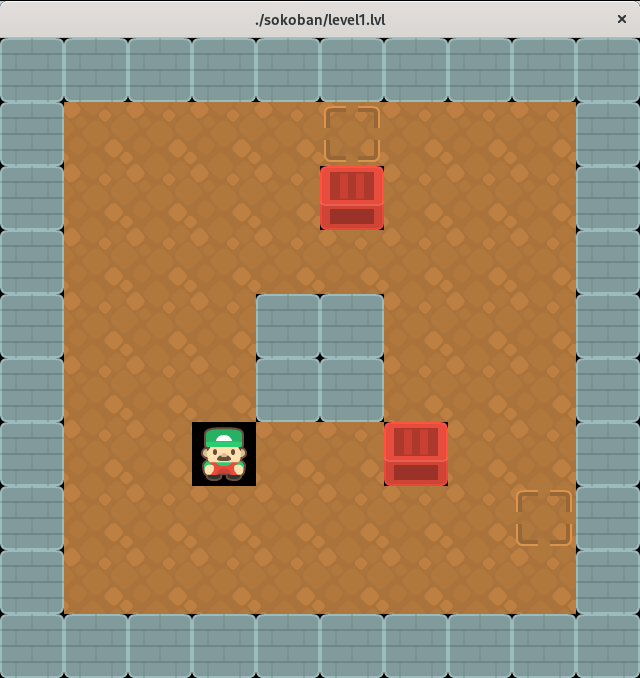
\includegraphics[width=1\textwidth]{projectPictures/PS2a.png}
    \label{fig:ps2a}
\end{figure}

